\documentclass[12pt,a4paper]{article}
\usepackage[left=3cm,right=1cm,top=2cm,bottom=2cm]{geometry}

\usepackage[T2A]{fontenc}
\usepackage[utf8]{inputenc}
\usepackage[russian,english]{babel}

\usepackage{indentfirst}
\usepackage{graphicx}
\graphicspath{ {./res/} }
\usepackage{caption}
\usepackage{subcaption}
\captionsetup[figure]{name={Рис.}}
\usepackage{listings}
\usepackage{float}
\usepackage{enumitem}

\setlist[enumerate]{label*=\arabic*.}

\begin{document}
\begin{titlepage}

\thispagestyle{empty}

\centerline{Лицей НИУ ВШЭ}

\vfill

\centerline{\large{\textsc{\textbf{Рендеринг трехмерных объектов}}}}
\centerline{\large{\textsc{\textbf{методом ray marching}}}}

\vfill

Ученик группы 9ФМ \hfill Чубий Савва Андреевич

\vfill

\centerline{Москва, 2020}
\clearpage
\end{titlepage}
\sloppy


\section{Цель использования метода}
Данный метод используется для получения двумерной проекции трехмерных объектов
на плоскоси с последующим отображением плоскости на экране.


\section{Signed Distance Function}
Для использования ray marching-а необходимо знать $sdf$ для объектов сцены.
$sdf$~(Signed Distane Function, знаковая функция расстояния) --- функция,
возвращающая минимальное расстояние от данной точки в пространстве до
поверхности объекта, который требуется изобразить.
\begin{itemize}
    \item $sdf(P) > 0$, если точка $P$ расположена вне объекта.
    \item $sdf(P) = 0$, если $P$ лежит на поверхности.
    \item $sdf(P) < 0$, если $P$ находится внутри объекта.
\end {itemize}
\vspace{\baselineskip}

Для большего понимания выведем формулу $sdf(P)$ для шара.
\begin{enumerate}
    \item Пусть центр шара расположен в точке $C$, а его радиус равен $r$.
    \item Минимальное расстояние от $P$ до поверхности шара равно длине
        перпендикуляра, опущенного из $P$ на поверхность шара. Назовем этот
        перпендикуляр $PH$
    \item $CP = PH + CH  \ \Rightarrow \  sdf(P) = CP - PH = \left|P - C\right| - r  
        \ \Rightarrow \  sdf(f) = \left|P - C\right| - r$
\end{enumerate}
% \begin{figure}[h!]
%     \centering
%     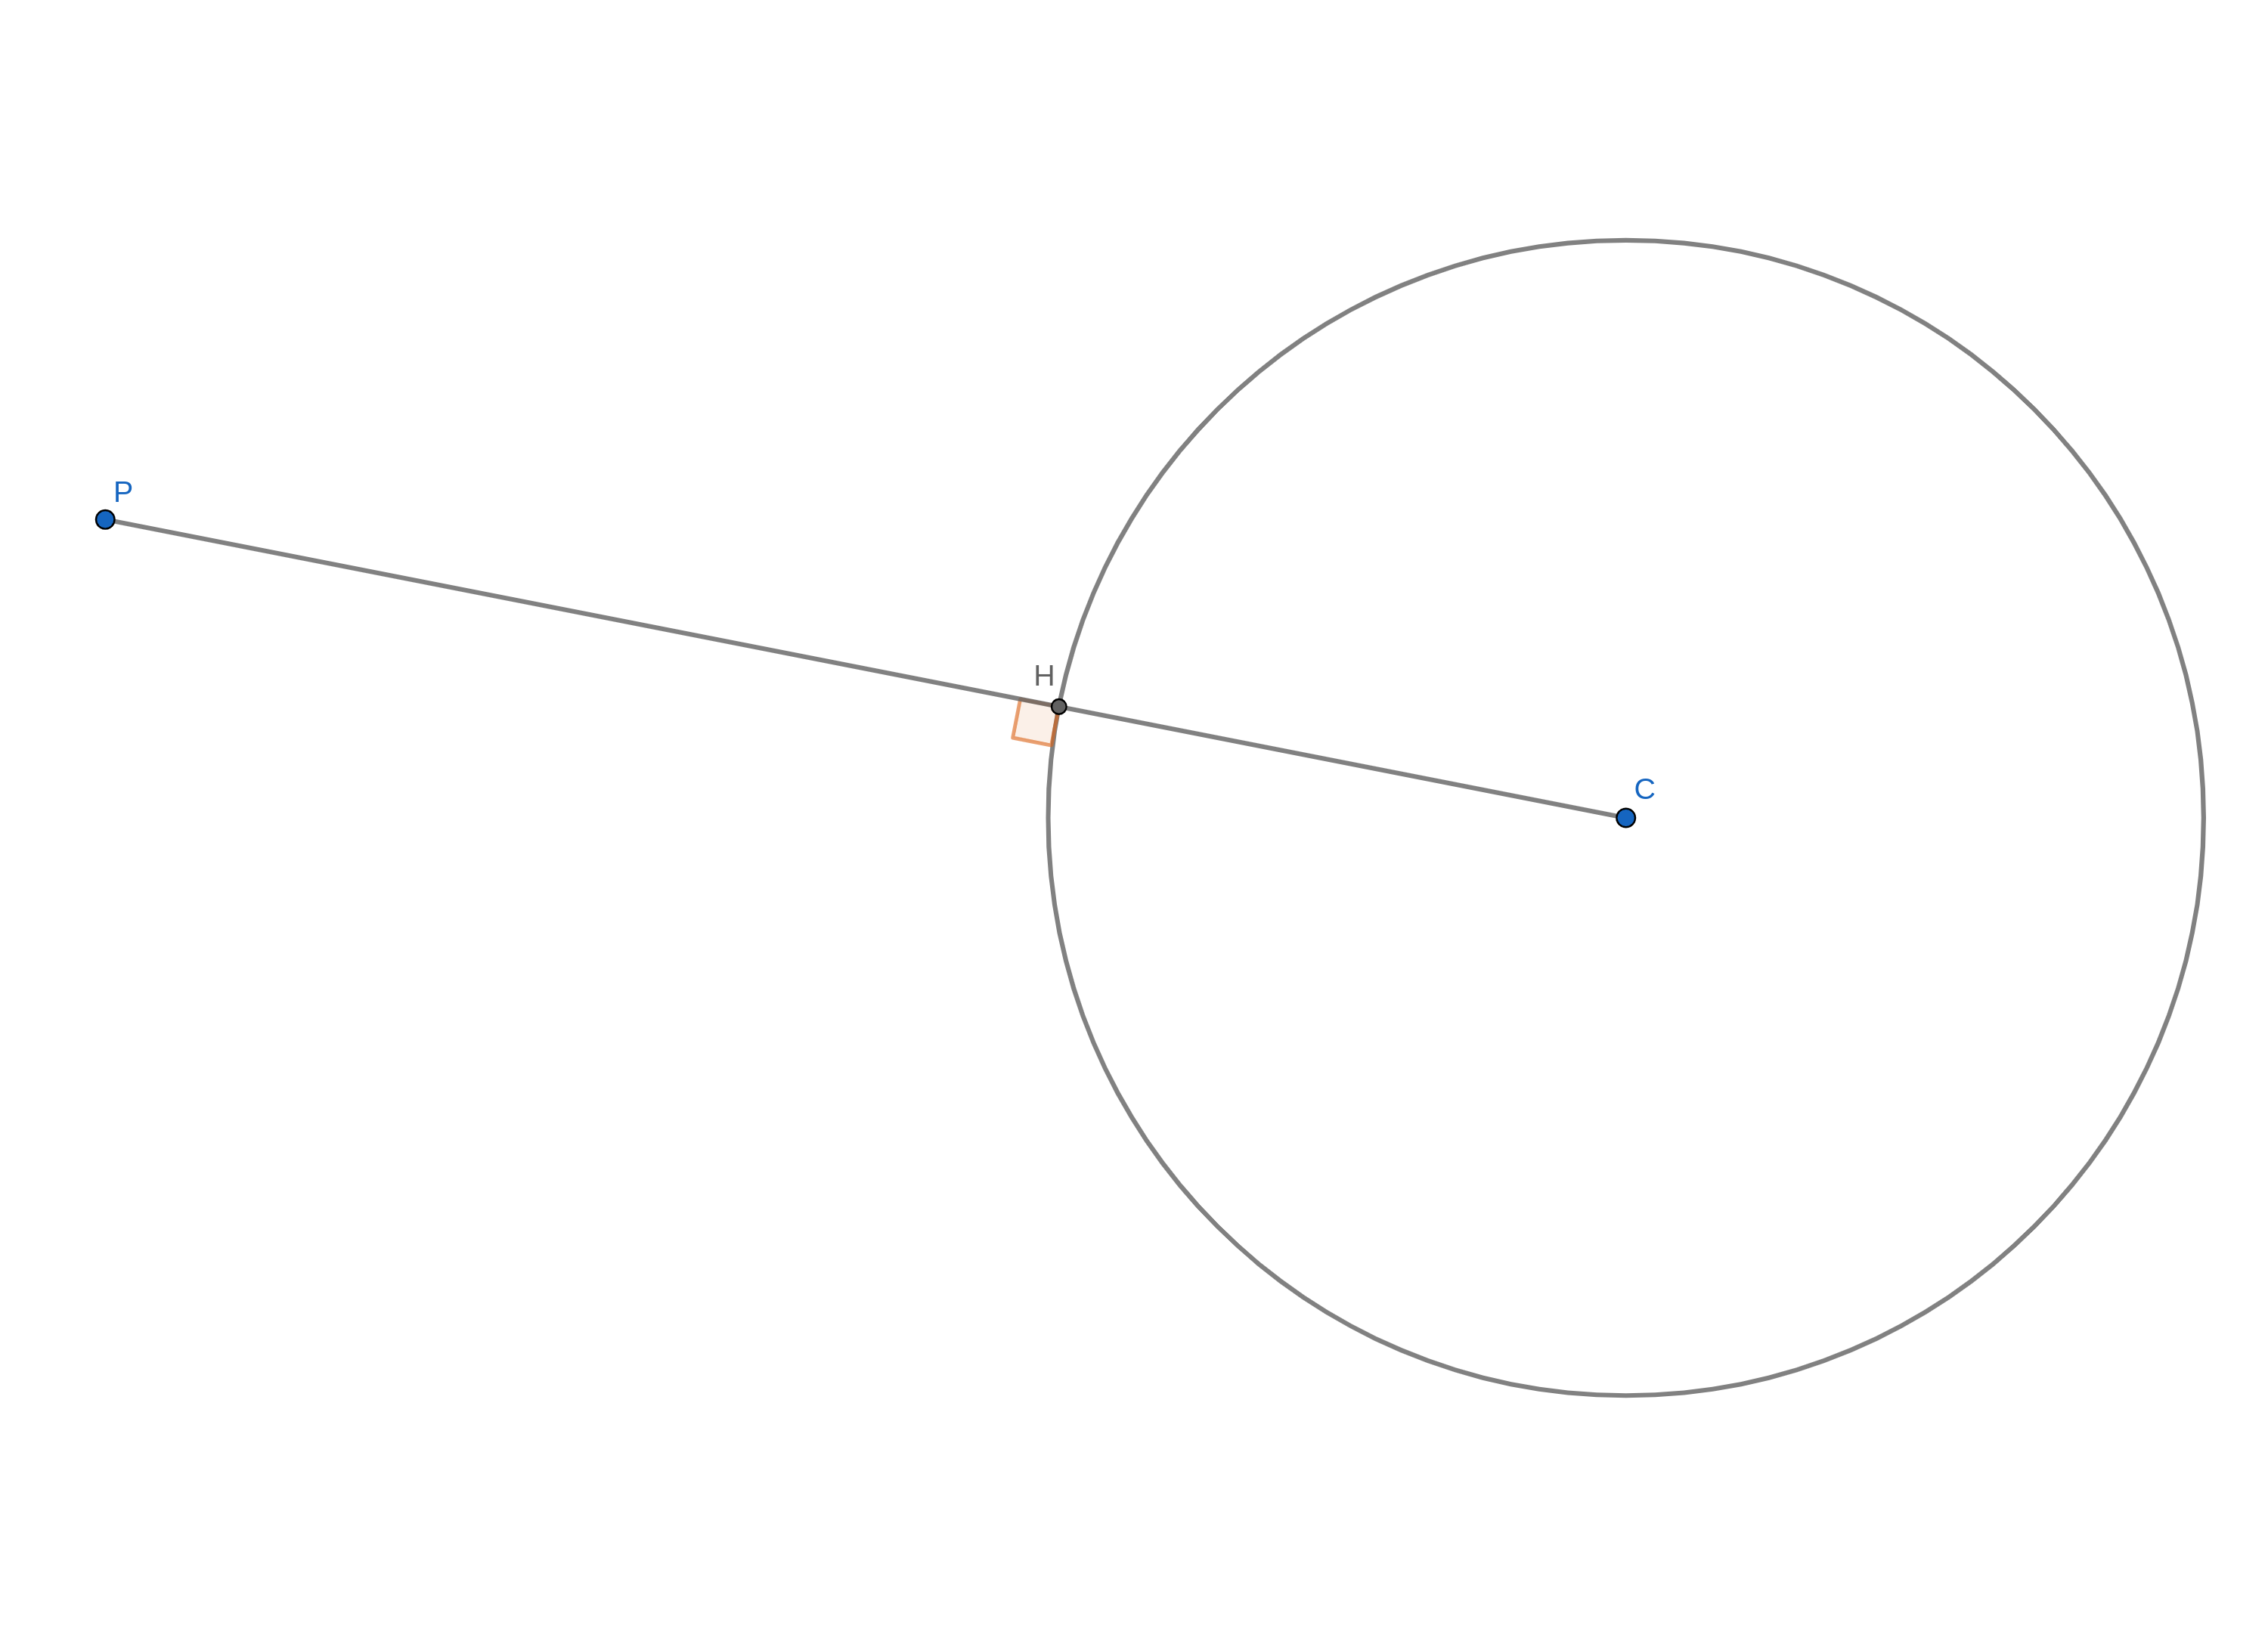
\includegraphics[height=5cm]{circle_SDF}
%     \caption{Чертеж к задаче вывода $sdf$ шара}
% \end{figure}

Такую функцию можно найти не только для шара, но и для куба, конуса, капсулы, 
тора, цилиндра и некоторых других фигур. Также $sdf$ можно преобразовывать: 
округлить края, отразить или выгнуть фигуру, повторить её бесконечное
количество раз и т.д.


\section{Принцип работы}
Нам дана точка $C$ (от Camera) --- расположение камеры, и единичные векторы
$\vec{f}$ (от front), $\vec{r}$ (от right), $\vec{u}$ (от up), указывающие
вперед, вправо и вверх соответственно, относительно направления камеры.
($\vec{f} \perp \vec{r}, \vec{r} \perp \vec{u}, \vec{u} \perp \vec{f}$)

Перед камерой расположенная плоскость, на которой отмечен прямоугольник.
Плоскость и $\vec{f}$ перпендикулярны, две смежные стороны прямоугольника
параллельны $\vec{u}$ и $\vec{r}$ соответственно, а луч сонаправленный
$\vec{f}$, начинающийся в $C$, пересекает прямоугольник в его центре. Этот
прямоугольник как бы является нашим монитором.

Теперь мы хотим получить цвет каждого пикселя. Для этого пропустим через точку
на прямоугольнике, соответствующую данному пикселю луч, начинающийся в $C$. Луч
будет сонаправлен вектору $uv_x \cdot \vec{r} + uv_y \cdot \vec{u} + \vec{f}$,
где $\vec{uv}$ --- двумерный вектор, описывающий координату пикселя.
($\vec{uv} = \left(0, 0\right)$ в центре экрана.) Если луч попал в какой-либо
объект, красим пиксель в цвет этого объекта, иначе пиксель будет цвета заднего
фона.

\begin{figure}[H]
    \centering
    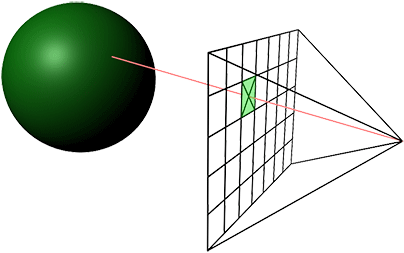
\includegraphics[height=6cm]{get_pixel}
    \caption{Получение цвета пикселя}
\end{figure}

Осталось понять, каким образом проверяется пересечение луча и объекта, заданного
$sdf$. Важно заметить, что именно эта часть отличает ray marching от похожих
методов, например, ray tracing-а.
\begin{enumerate}
    \item Рассматривается луч, заданный точкой начала $ro = C$ и
        направлением $\vec{rd} = normalize(uv_x \cdot \vec{r} + uv_y \cdot
        \vec{u} + \vec{f})$.
    \item Работа алгоритма состоит из нескольких итераций, количество которых
        задается заранее. Чем больше итераций --- тем лучше изображение и
        медленнее программа.
    \item Будем "шагать" по лучу, пока не доберемся до объекта. Один шаг ---
        одна итерация.
    \item Пусть $t_0 = 0$, где $t_i$ --- расстояние, пройденное по лучу к $i$-ой
        итерации.
    \item Рассмотрим $i$-ую итерацию.
    \begin{enumerate}
        \item Найдем точку, в которой мы находимся: $P_i = \vec{ro} + t_i
            \cdot \vec{rd}$
        \item Вычислим минимальное расстояние от неё до объектов сцены $h_i =
        sdf\left(P_i\right)$
        \item Если это расстояние меньше некоторого порога, то считаем, что
            добрались до объекта и завершаем алгоритм. Порог задается заранее.
            Чем он меньше, тем лучше изображение.
        \item Если мы продвинулись по лучу дальше некоторого расстояния,
            выбранного заранее, говорим, что ни с чем не пересеклись и завершаем
            алгоритм. Ограничение дальности прорисовки устанавливается для
            ускорения работы программы.
        \item "Шагаем" по лучу $t_{i + 1} = t_i + h_i$. Т.к. $h_i$ минимальное
            расстояние, то мы точно не "перешагнем" через какой-то объект.
    \end{enumerate}
    \item Будем считать, что пересеклись с объектом, который ближе всего к
        $P_{last}$. При хорошо подобранных параметрах до этой части мы будем
        доходить только в тех случаях, когда луч почти пересекает объект,
        поэтому разумно считать, что мы его пересекли.
\end{enumerate}
\begin{figure}[H]
    \centering
    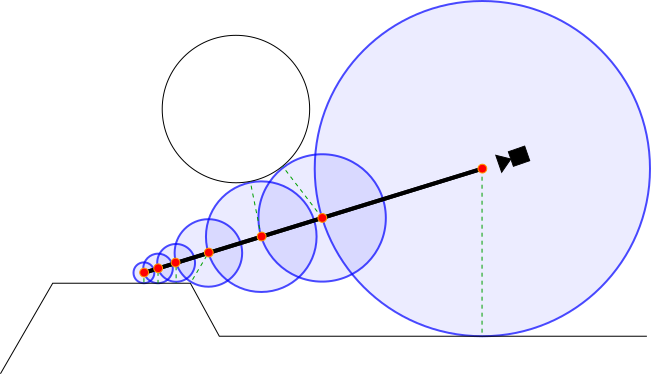
\includegraphics[height=6cm]{marching_principle}
    \caption{Принцип работы ray marching-а}
\end{figure}


\section{Программная реализация}
Покажем реализацию данного алгоритма на языке программирования glsl. Полные
коды программ, используемых для генерации некоторых изображений ниже,
приводиться не будут по причине больших размеров и простоты их написания.
\begin{lstlisting}[language=c++]
float marching(in vec3 ro, in vec3 rd) {
    float t = 0.;
    for (float i = 0.; i < MARCHING_ITERATIONS; ++i) {
        vec3 P = ro + rd*t;

        float h = sdf(P);
        if (h < RAY_INTERSECTION_TRASHOLD)
            break;
        if (t > ZFAR)
            break;
        t += h;
    }
    if (t > ZFAR) t = inf;
    return t;
}
\end{lstlisting}

\begin{figure}[H]
    \centering
    \begin{subfigure}{0.5\textwidth}
        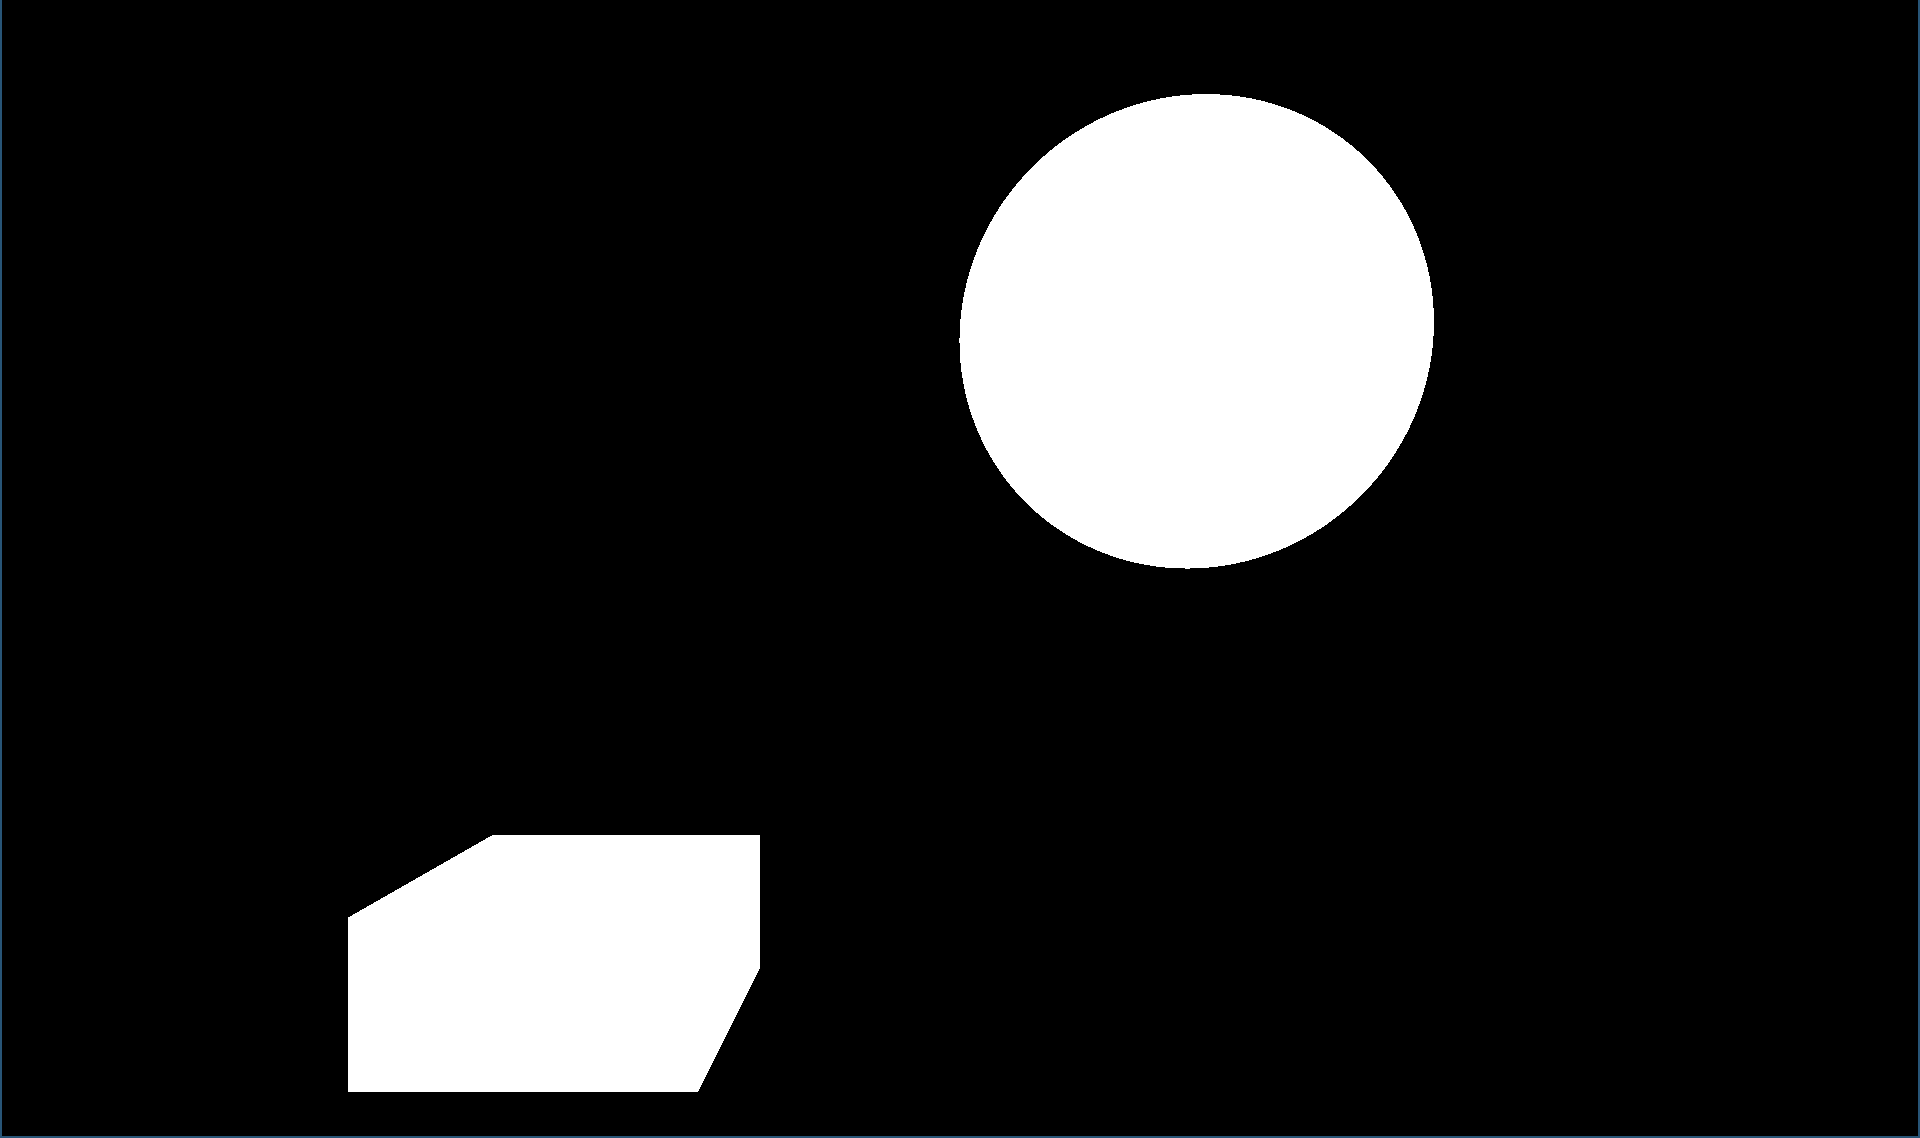
\includegraphics[width=0.9\textwidth]{no_light_screenshot}
    \end{subfigure}%
    \begin{subfigure}{0.5\textwidth}
        
\includegraphics[width=0.9\textwidth]{no_light_screenshot2}
    \end{subfigure}
    \caption{Изображения, полученные методом ray marching-а (без освещения)}
    \label{img:no_light}
\end{figure}


\section{Освещение}
Как видно на рисунке \ref{img:no_light} трехмерные объекты выглядят
нереалистично. Проблема в том, что они не освещены, но это легко исправить.
Например, можно использовать модель освещения Фонга. Однако для этого необходимо
знать нормаль к поверхности фигур. Её легко вычислить, учитывая, что мы знаем
$sdf(P)$. $$\vec{n} = normalize\left(\frac{d \cdot sdf}{dx}, \frac{d \cdot sdf}{dy},
\frac{d \cdot sdf}{dz}\right)$$, где $\vec{n}$ --- вектор нормали к поверхности.
С освещением объекты выглядят значительно лучше. (См. рисунок \ref{img:with_light}.)

\begin{figure}[H]
    \centering
    \begin{subfigure}{0.5\textwidth}
        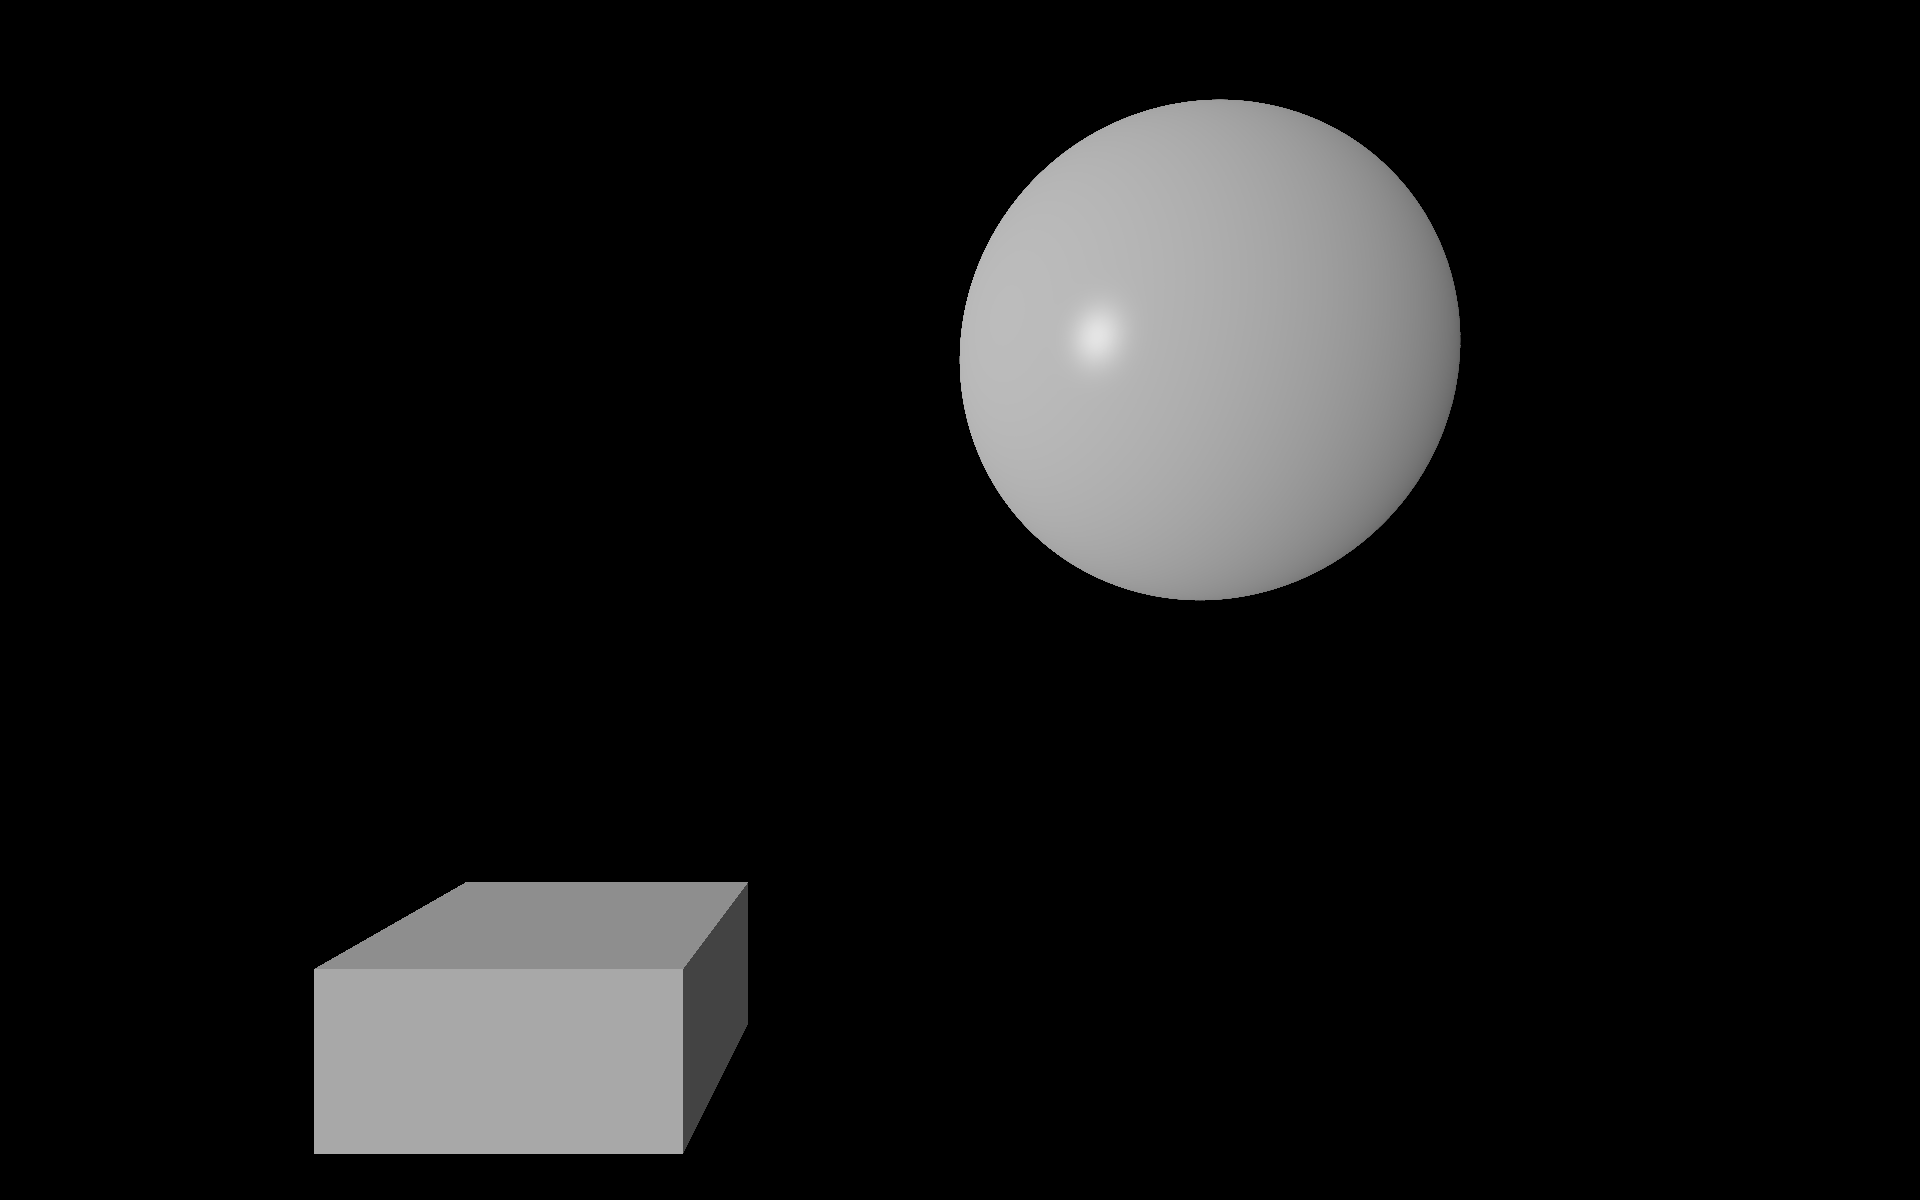
\includegraphics[width=0.9\textwidth]{with_light_screenshot}
    \end{subfigure}%
    \begin{subfigure}{0.5\textwidth}
        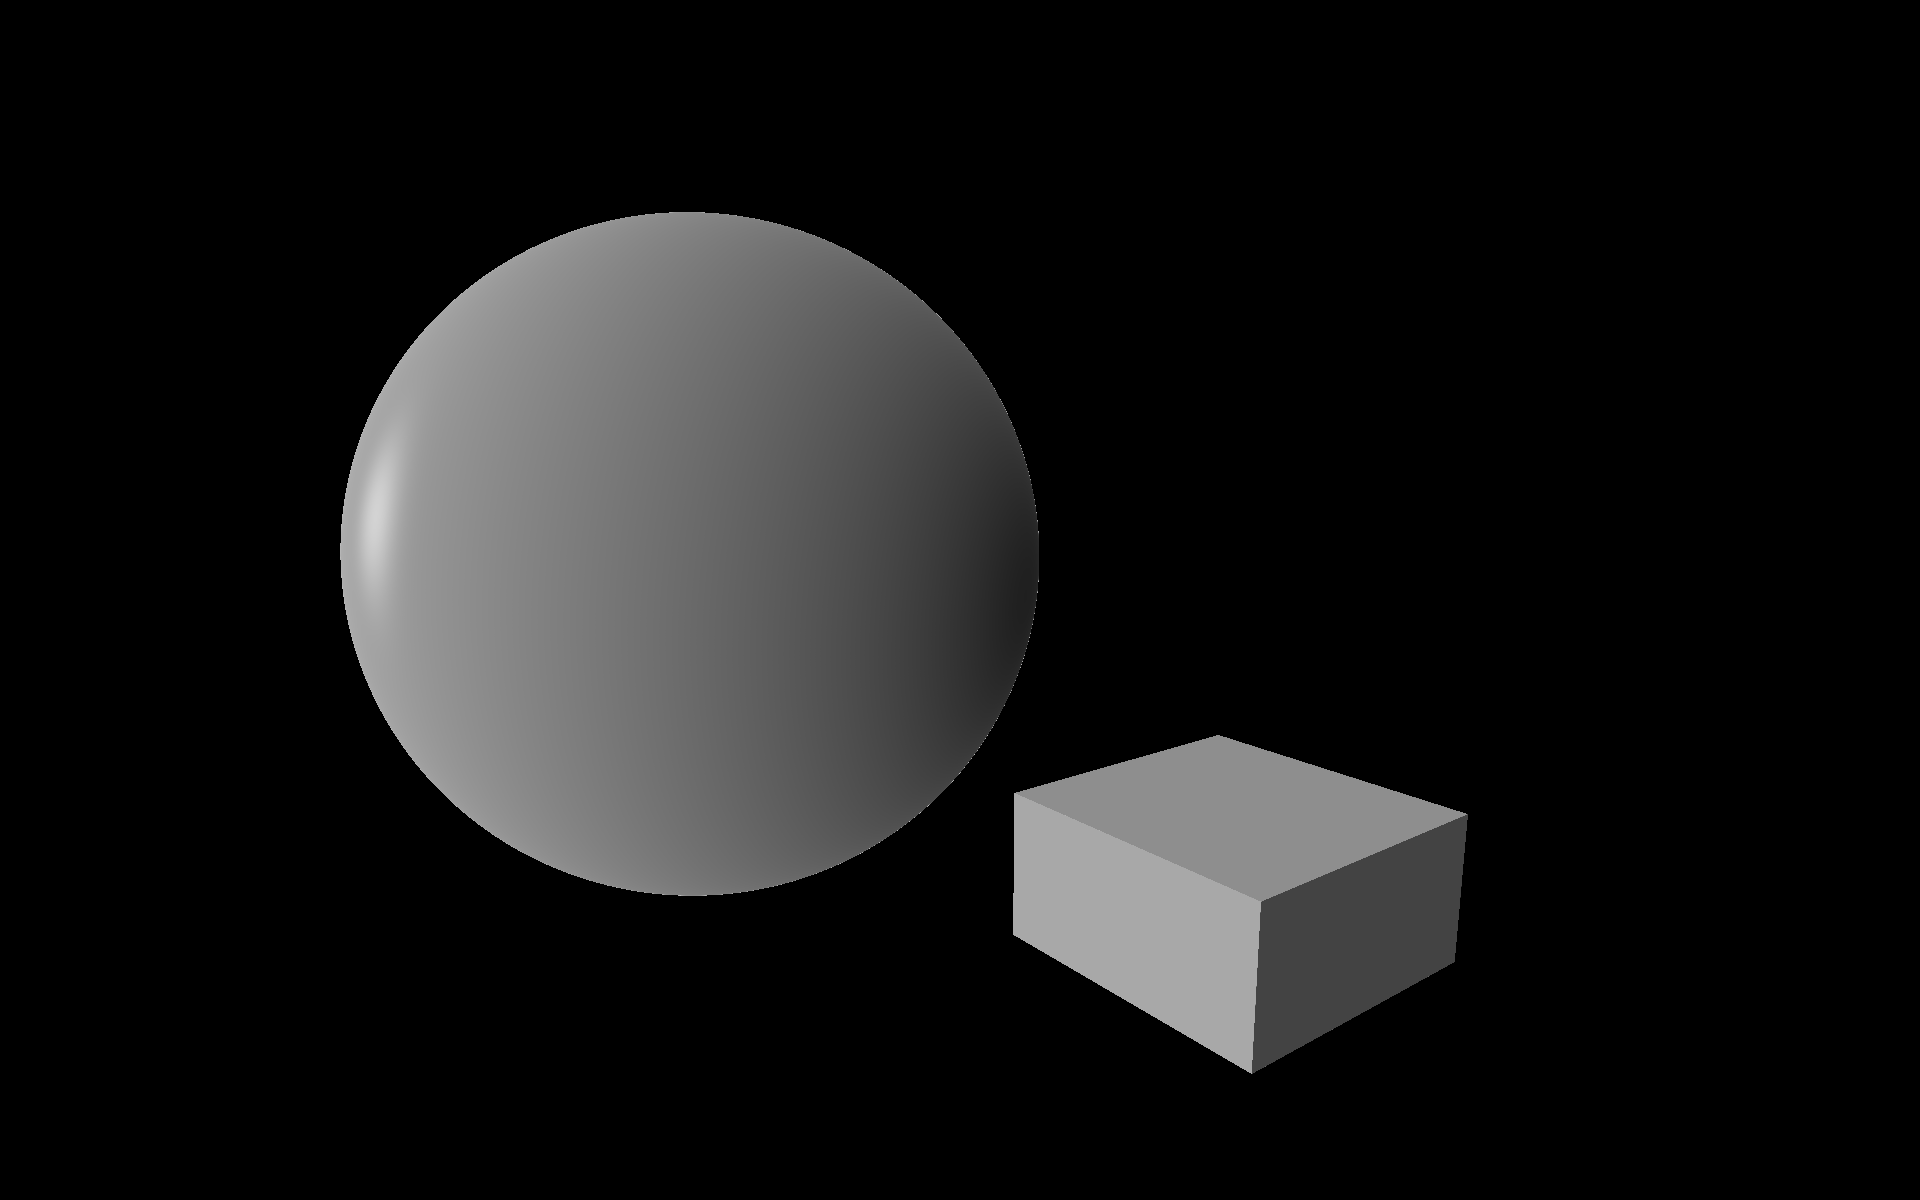
\includegraphics[width=0.9\textwidth]{with_light_screenshot2}
    \end{subfigure}
    \caption{Изображения, полученные методом ray marching-а (с освещением)}
    \label{img:with_light}
\end{figure}


\section{Преимущества и недостатки данного метода}
\subsection{Преимущества}
\begin{itemize}
    \item Достаточно быстрый для того, чтобы работать в реальном времени (при
        малом количестве объектов для отрисовки).
    \item Найти $sdf$ достаточно легко даже для сложных фигур, например,
        оболочки Мандельброта или проекций трехмерных объектов.
    \item Над $sdf$ просто производить различные преобразования: зеркально отражать
        масштабировать, изгибать и т.д.
    \item $sdf$ позволяет быстро считать нормаль к плоскости, что полезно для
        создания освещения.
\end{itemize}

\subsection{Недостатки}
\begin{itemize}
    \item Скорость работы алгоритма, а точнее скорость поиска значения $sdf$,
        быстро понижается при добавлении большого количества объектов,
        что, например, не позволяет использовать только ray marching при
        создании компьютерных игр.
\end{itemize}


\section{Галерея}
Здесь показаны несколько изображений, сгенерированных программами,
написанными мной с использованием мотода ray marching-а.

\begin{figure}[H]
    \centering
    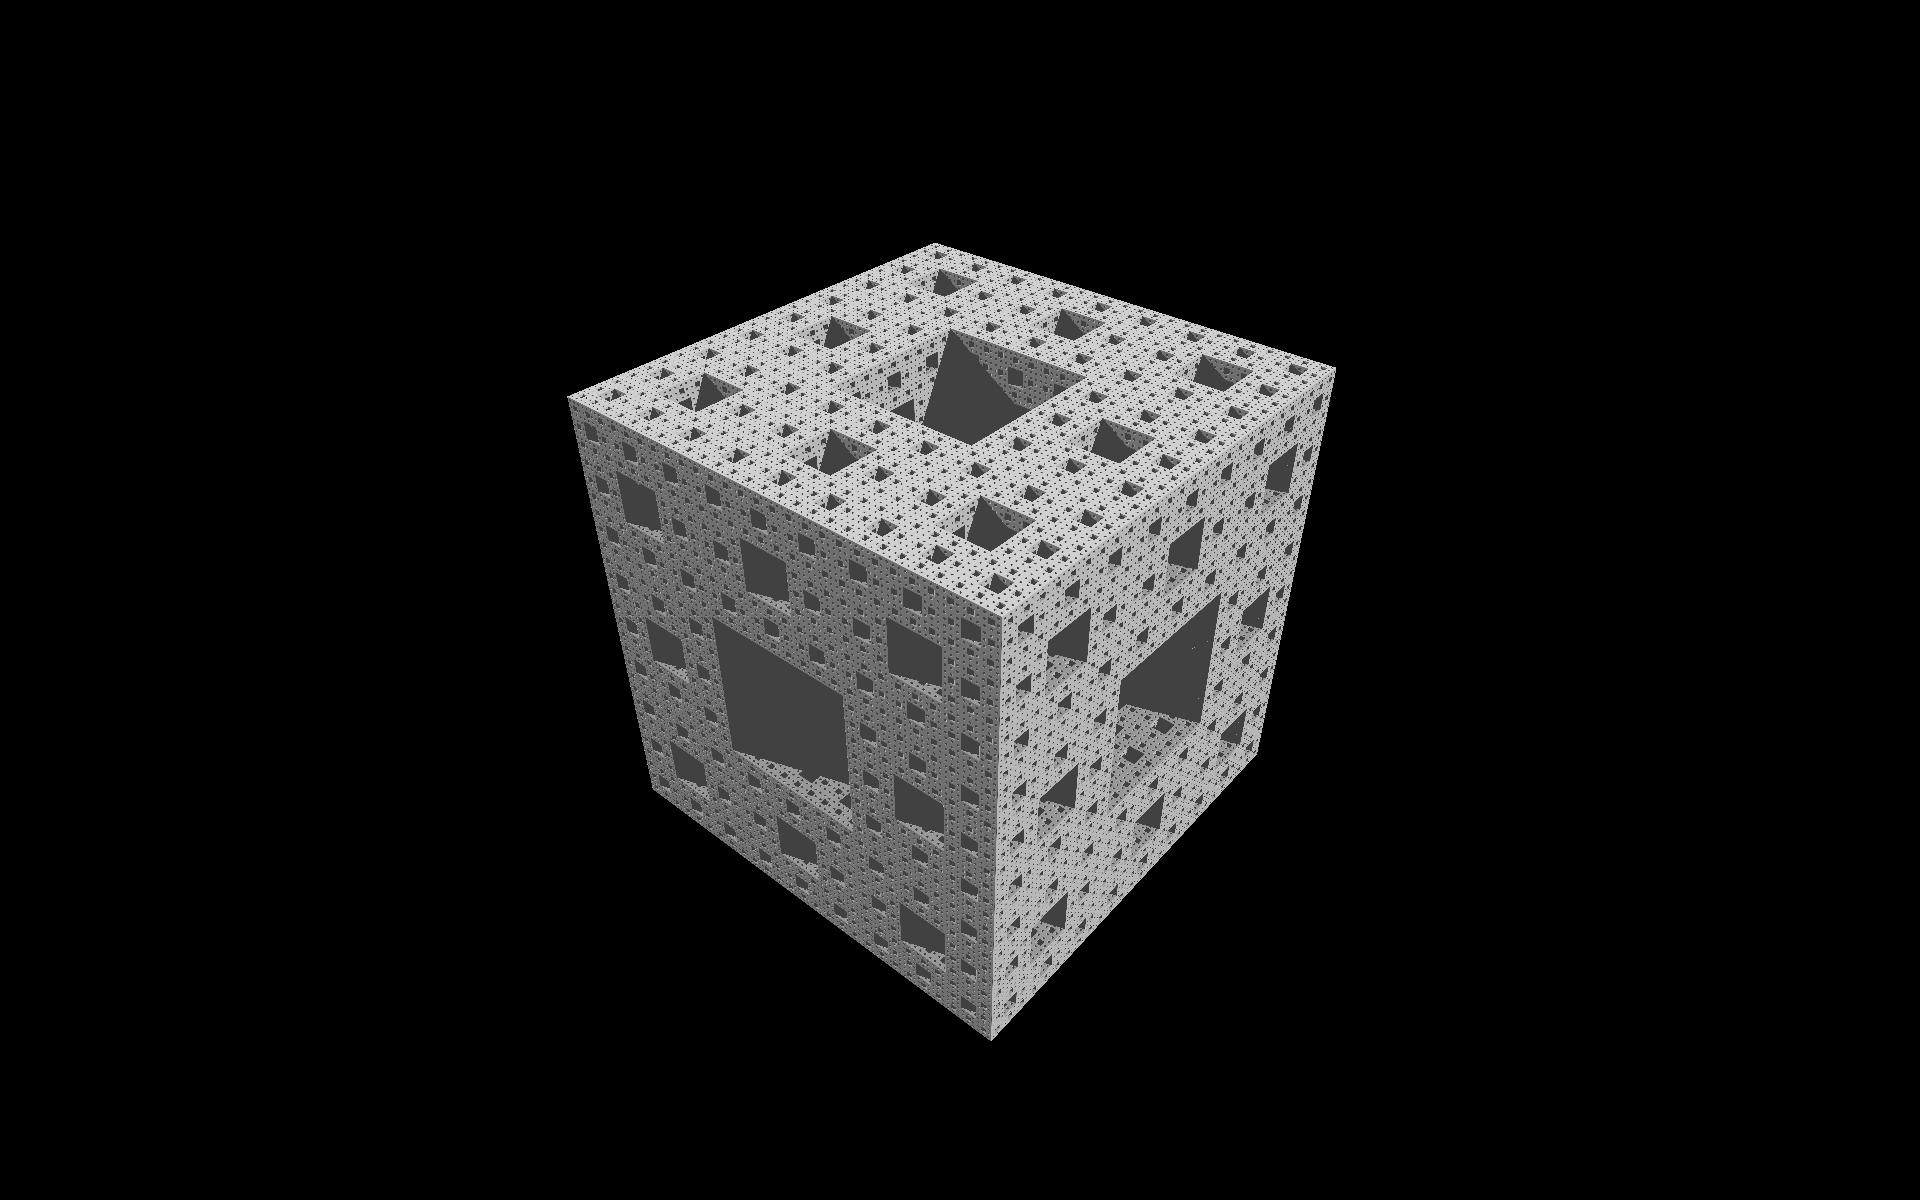
\includegraphics[width=\textwidth]{gallery2.png}
    \caption{Губка Менгера (вид снаружи)}
\end{figure}

\begin{figure}[H]
    \centering
    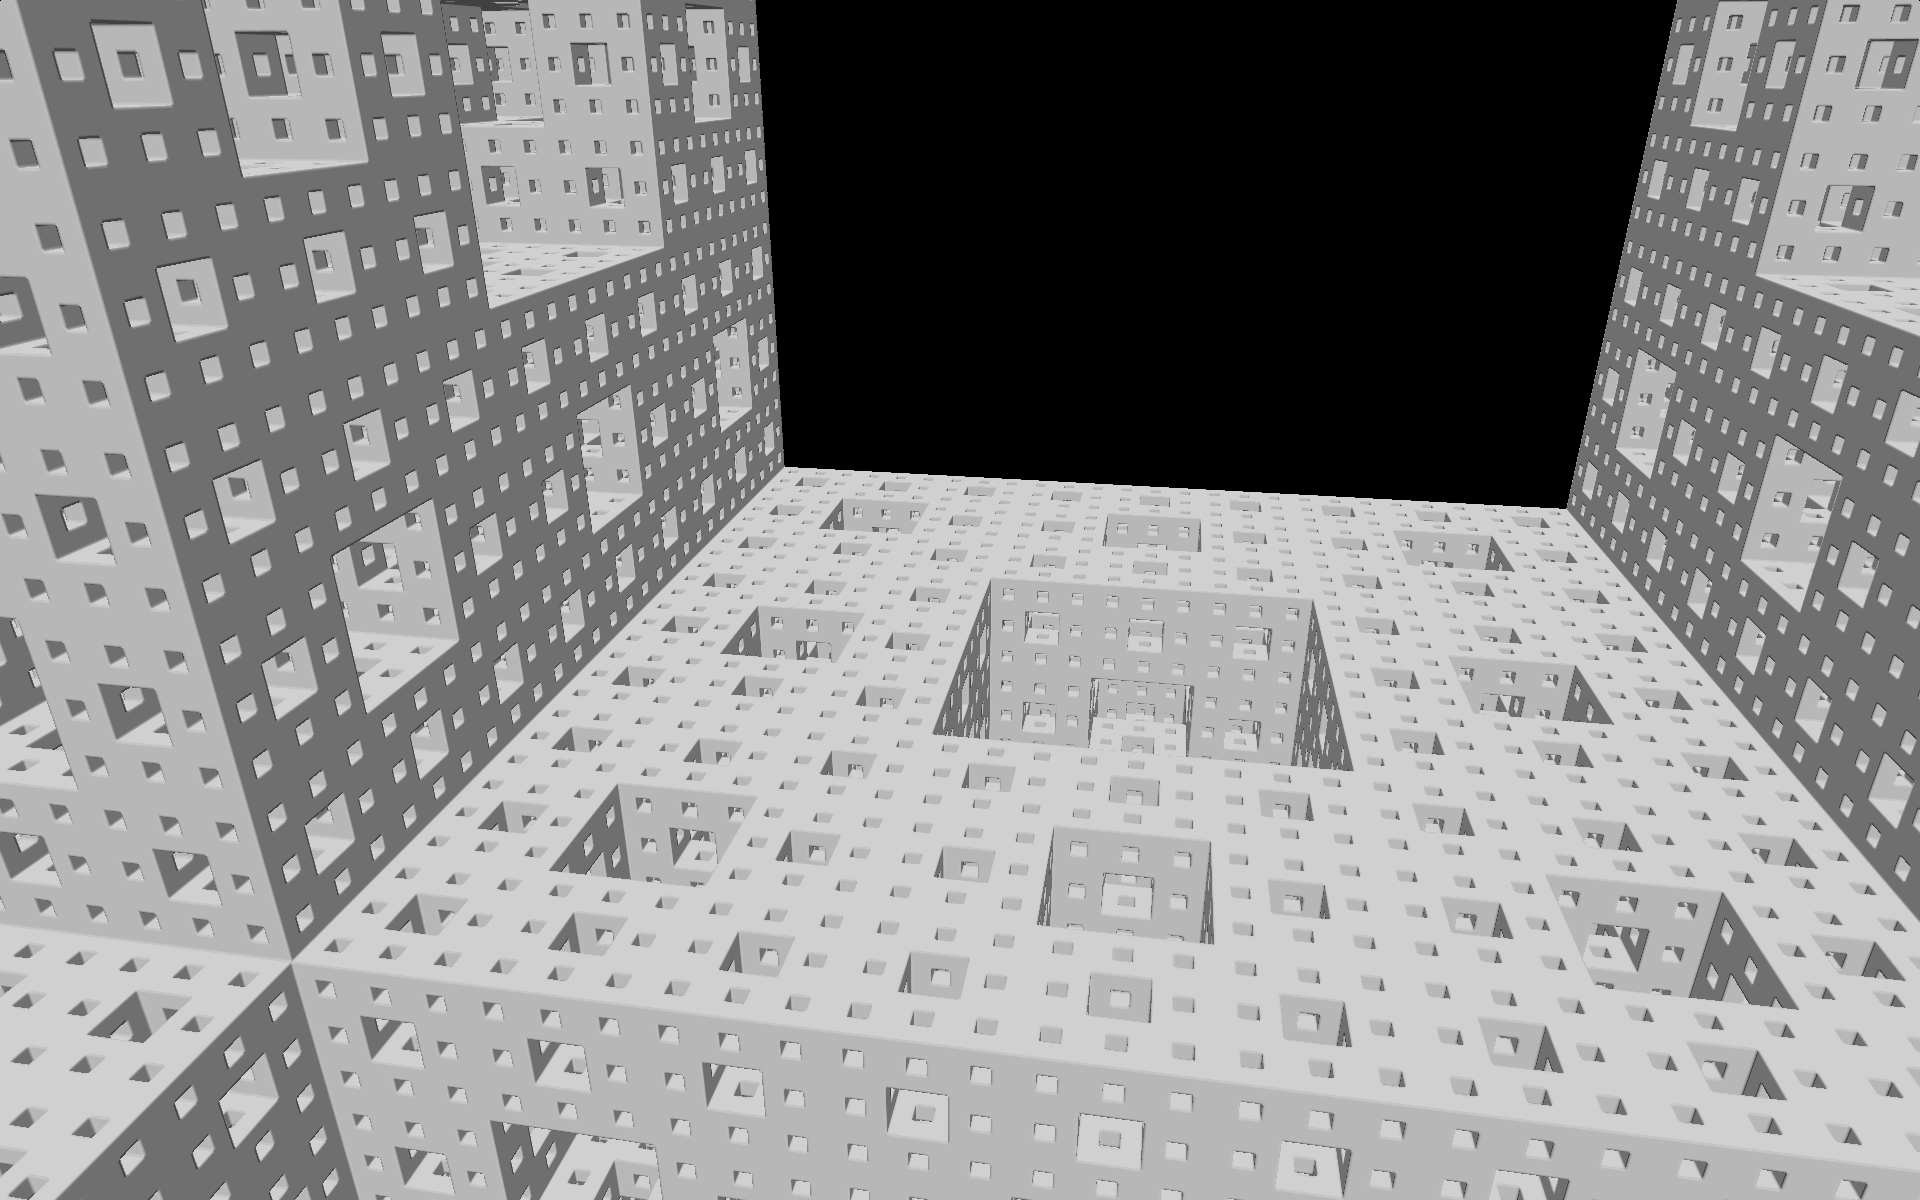
\includegraphics[width=\textwidth]{gallery3.png}
    \caption{Губка Менгера (вид изнутри)}
\end{figure}

\begin{figure}[H]
    \centering
    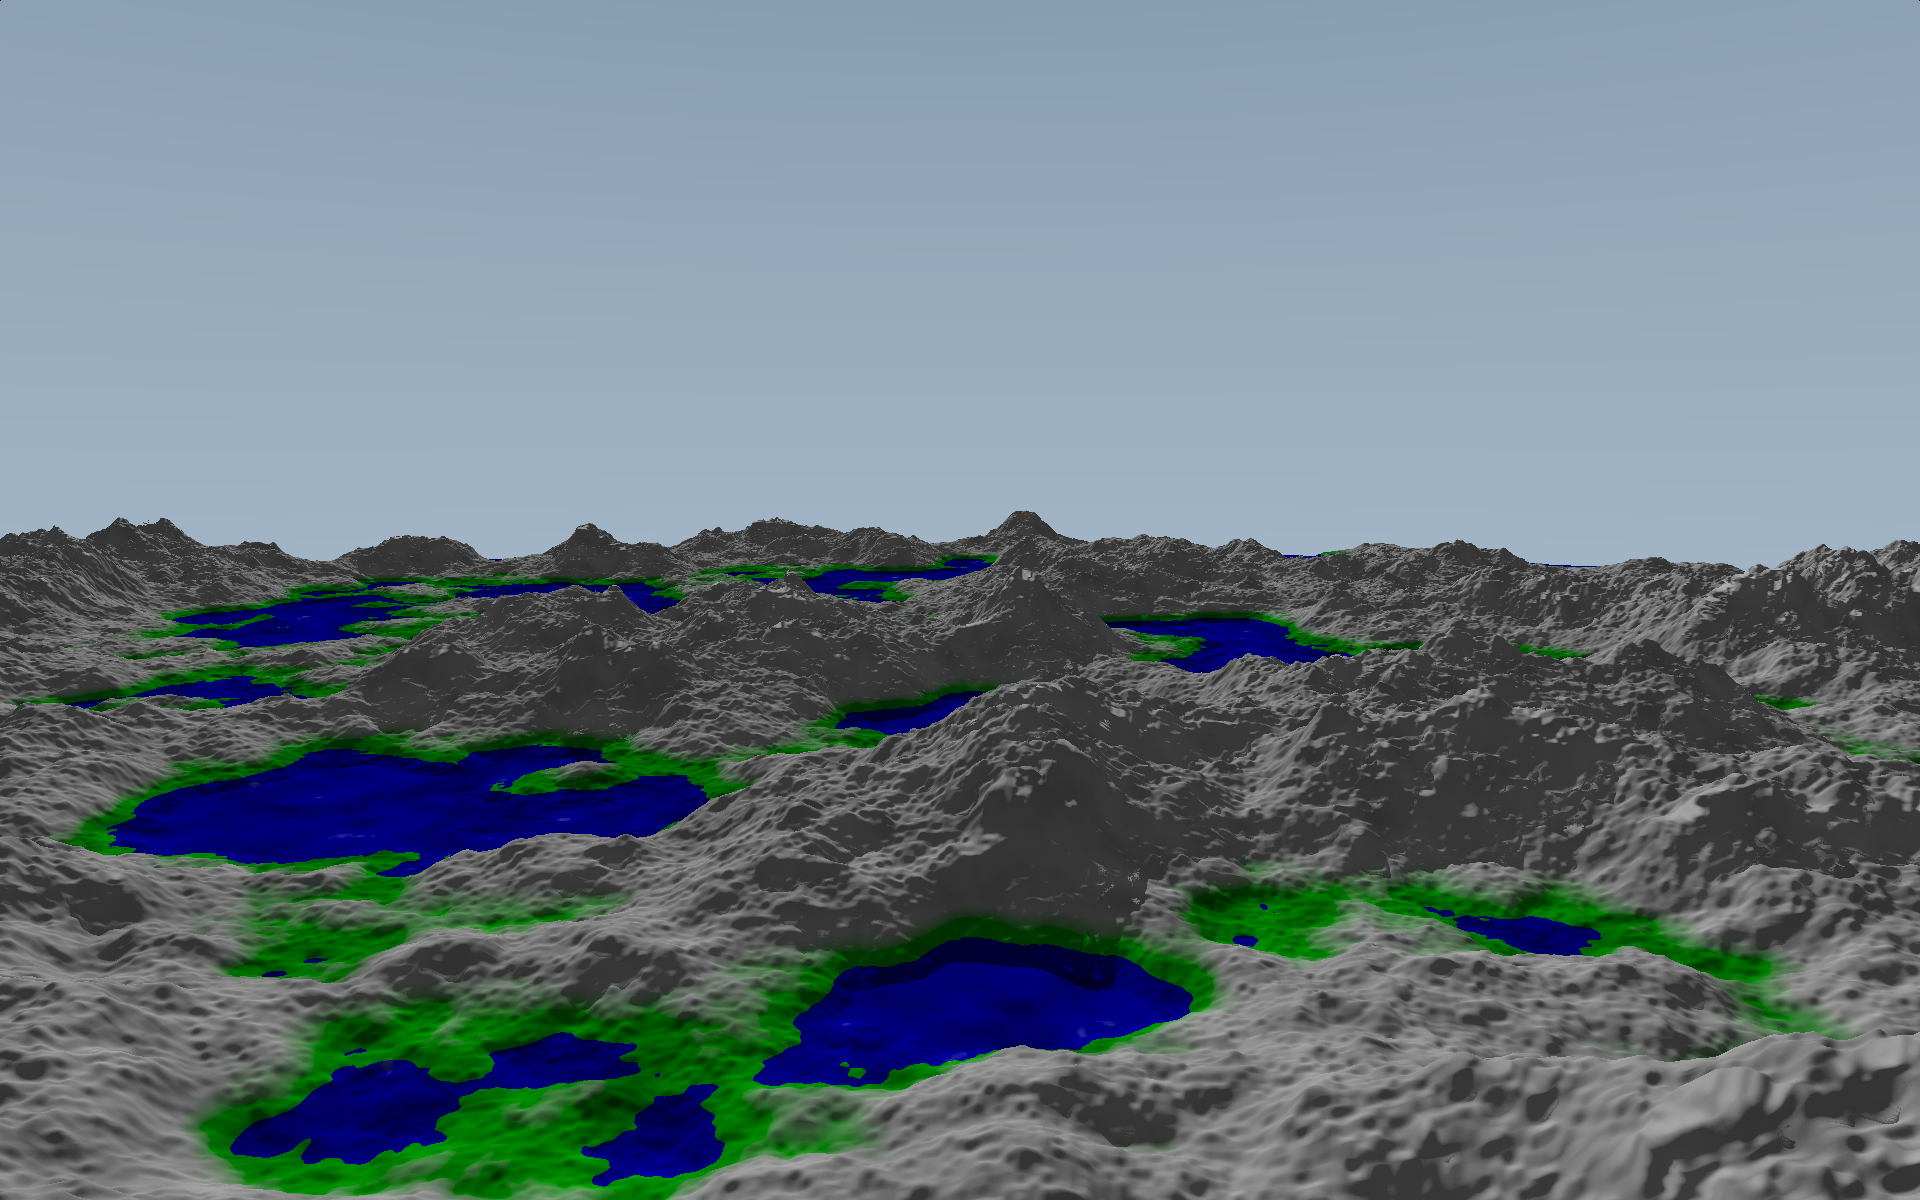
\includegraphics[width=\textwidth]{gallery1.png}
    \caption{Горный ландшафт (на основе шума Перлина)}
\end{figure}

\begin{figure}[H]
    \centering
    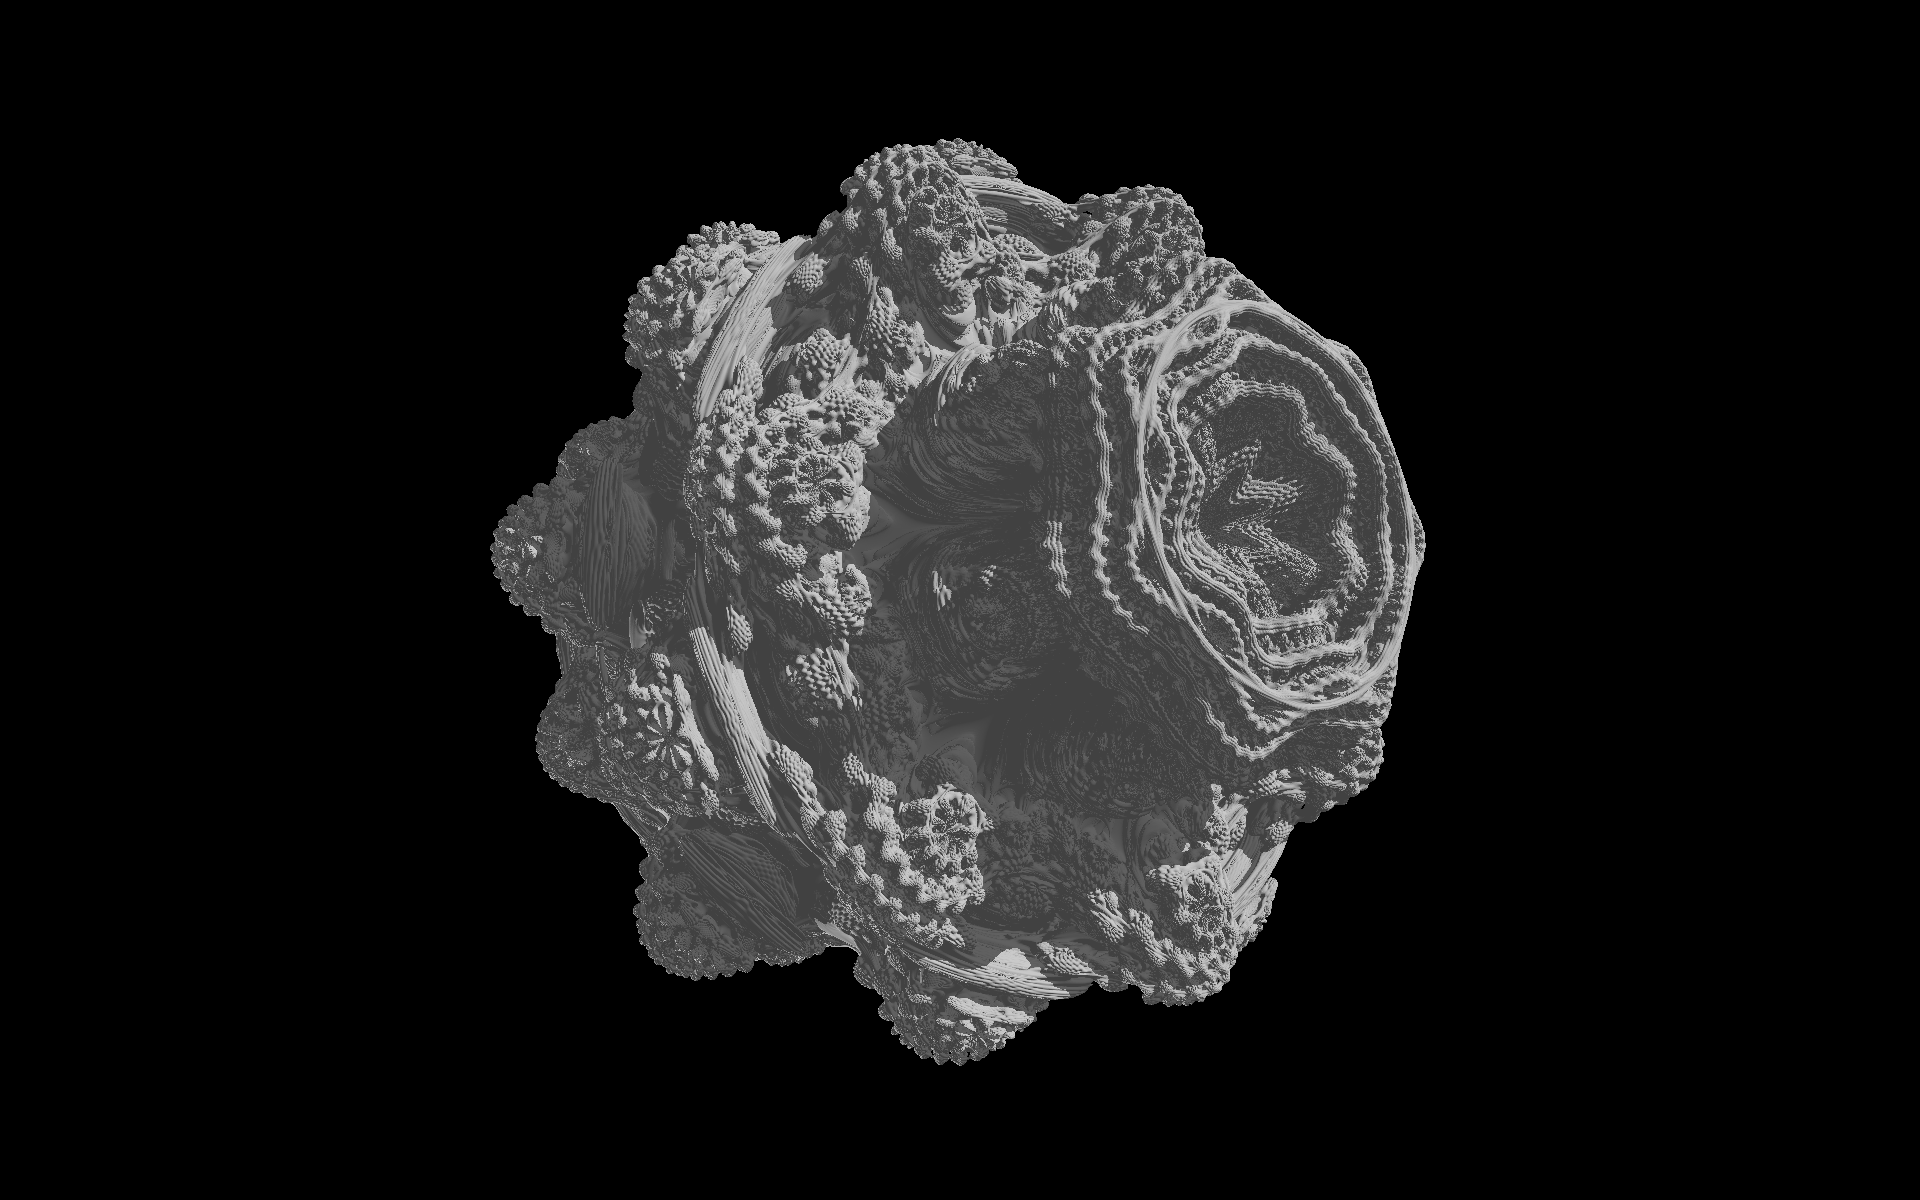
\includegraphics[width=\textwidth]{gallery4.png}
    \caption{Оболочка Мандельброта}
\end{figure}
\end{document}
